\chapter{L' Azienda}
    \section{SogeaSoft S.r.l}
    SogeaSoft S.r.l. è un'azienda di sviluppo \textit{software} fondata nel 1980 a Treviso, con l'obiettivo di progettare e realizzare soluzioni a supporto dei processi aziendali, servendo diverse realtà nel Triveneto.
    Oggi, SogeaSoft rappresenta una filiale di Bluenext S.r.l., azienda di consulenza informatica fondata nel 2012 a Rimini, attiva su tutto il territorio nazionale. Inizialmente, l'azienda acquisitrice si concentrava esclusivamente sullo sviluppo di un \textit{software} per ottimizzare il settore commerciale delle imprese, ma negli ultimi anni ha ampliato il proprio raggio d'azione, esplorando nuovi settori.
    
    \section{Organizzazione aziendale}
    La Figura 1.1 mostra come Sogeasoft S.r.l. sia strutturata in diverse aree operative, ciascuna dedicata alla gestione e allo sviluppo dei prodotti e servizi descritti nei punti seguenti: 
    
    \begin{itemize}
        \item \textbf{Sistema Aziendale Integrato - SAI}: si occupa dello sviluppo del \textit{software} gestionale \textit{Enterprise Resource $Planning_G$} ($ERP_G$), in particolare rappresenta la libreria di base e gestisce la contabilità.
        \item \textbf{SAICon}: sviluppa soluzioni verticali per il settore delle confezioni (abbigliamento) e calzaturiero, integrate con l'ERP SAI.
        \item \textbf{SAIOnWeb}: si concentra su applicativi correlati agli ERP, ma anche su soluzioni autonome come \textit{Customer Relationship $Management_G$} ($CRM_G$), \textit{Supplier Relationship \\
        $Management_G$} ($SRM_G$), raccolta ordini e \textit{After Sales $Service_G$} ($ASS_G$), ossia una serie di strumenti per ottimizzare le relazioni con i clienti e con i fornitori. Inoltre, sviluppa la nuova architettura per la migrazione del gestionale.
        \item \textbf{SAIPro}: fornisce applicativi per la pianificazione e il controllo della produzione, destinati alle aziende manifatturiere.
        \item \textbf{BI}: Sviluppa soluzioni per la \textit{$Business Intelligence_G$} ($BI_G$), focalizzandosi sull'analisi dei dati aziendali per ottimizzare le \textit{performance} e supportare decisioni strategiche più informate e mirate. 
        \item \textbf{CS} (\textit{Customer $Service_G$}): offre supporto ai clienti prima, durante e dopo l'acquisto tramite un ufficio dedicato a SAI e un altro dedicato a SAICon, per garantire assistenza costante.
        \item \textbf{Ufficio sistemistico}: si occupa della gestione dell'infrastruttura \textit{hardware}, sia interna all'azienda che per i clienti che richiedono supporto, oltre a fornire assistenza ai \textit{team} di sviluppo.
    \end{itemize}
    
    \noindent SAIonWeb è stato il tema principale del mio \textit{stage}. Il nome SAIonWeb era inizialmente legato al progetto originale, focalizzato esclusivamente su applicativi utilizzabili tramite il \textit{web}. Tuttavia, con l'evoluzione dell'architettura del sistema, il nome è diventato fuorviante. Attualmente il progetto si occupa di sviluppare un'infrastruttura più moderna e flessibile, che possa eventualmente supportare e gradualmente sostituire il gestionale SAI. 
    Questo processo prevede la collaborazione di membri provenienti da diverse aree, tra cui il \textit{team} di SAICon e quello di SAIPro, che lavorano congiuntamente per integrare i vari componenti del sistema.\\

    \begin{figure}
        \centering
        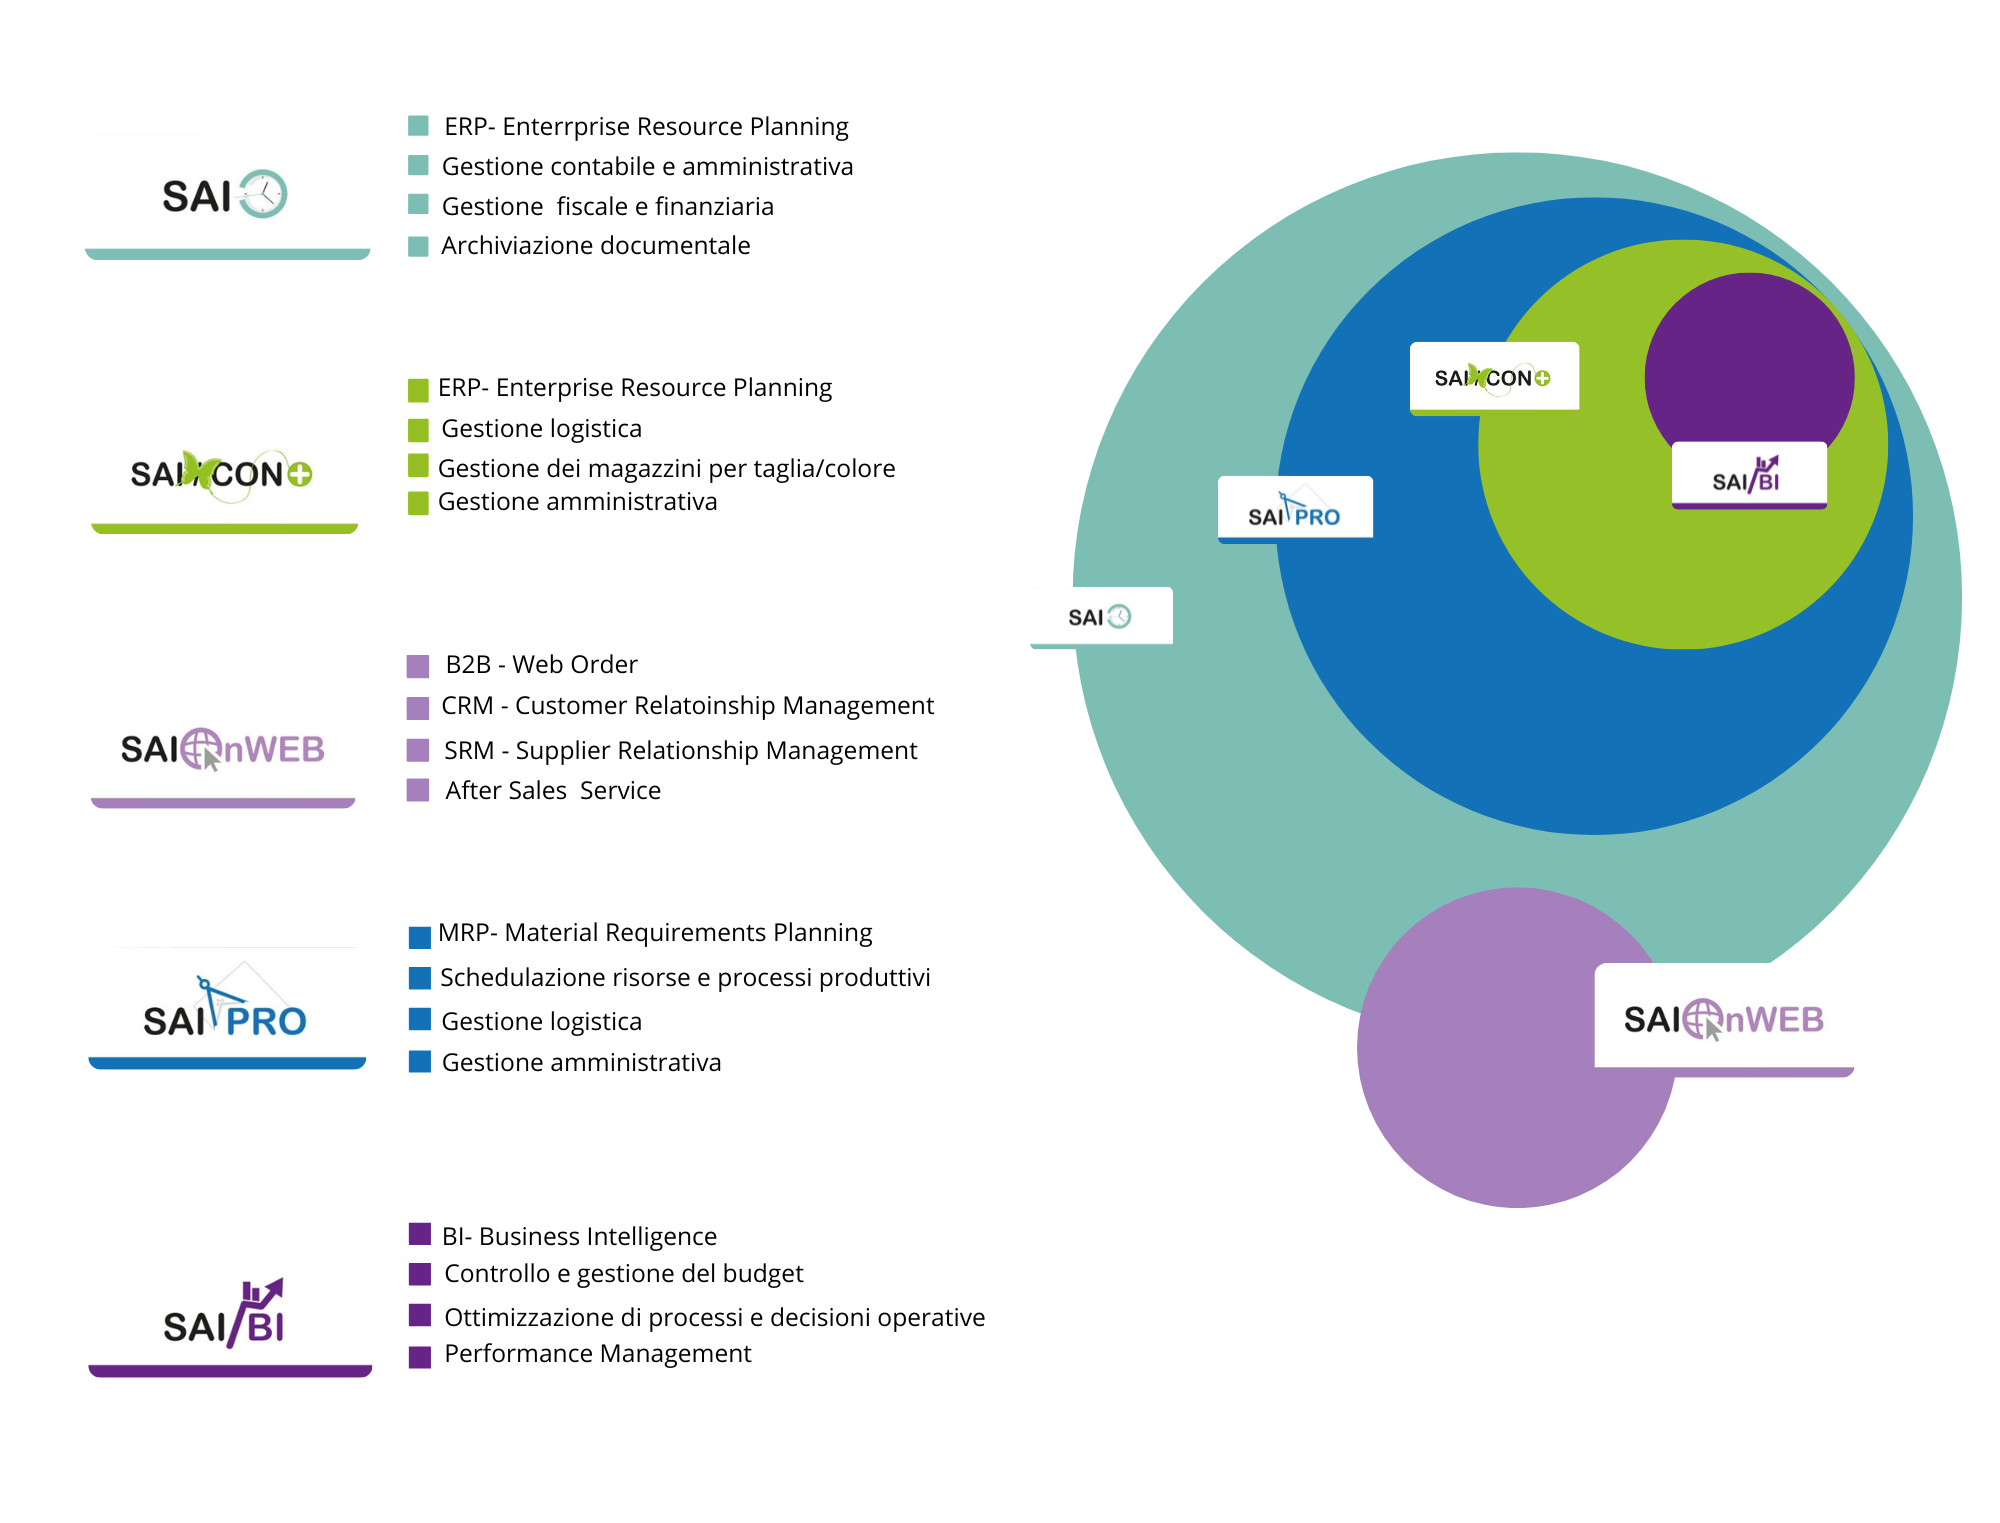
\includegraphics[width=0.9\linewidth]{BCS-Tessi/images/SOGEAProdotti.png}
        \caption{Panoramica dei prodotti e servizi offerti da SogeaSoft}
        \label{fig:panoramica_prodotti}
    \end{figure}

    \noindent Come si può osservare in Figura 1.1, i principali prodotti di SogeaSoft S.r.l. sono strettamente interconnessi, il che si riflette nell’organizzazione dei \textit{team} all’interno dell’azienda. Sebbene esista una divisione indicativa basata sul tipo di prodotto sviluppato, i ruoli risultano essere sfumati e coprono più aree di competenza. 
    \noindent Le persone che lavorano su ciascun prodotto fanno riferimento a un \textit{Product Owner}, che può rappresentare più \textit{team} in base alle necessità.

    \noindent Durante il mio \textit{stage} ho avuto modo di interagire con: 
    \begin{itemize}
        \item \textbf{\textit{Product Owner}}:è la figura responsabile della definizione delle caratteristiche di un prodotto, della gestione delle priorità e della comunicazione con il \textit{team} di sviluppo, al fine di garantire che il prodotto finale soddisfi le esigenze degli utenti e gli obiettivi aziendali;
        
        \item \textbf{\textit{Team Leader}}: gestisce il \textit{team} di sviluppo. In SogeaSoft S.r.l. questa figura può coincidere con il \textit{Product Owner} e/o con il \textit{Scrum Master} (approfondito nella Sezione 1.4);
        \item \textbf{Sviluppatore}: si occupa di progettazione, sviluppo e \textit{testing} del \textit{software}. In base al grado di esperienza contribuisce anche all'analisi e all'assistenza ai clienti. 
    \end{itemize}


    \section{Prodotti di SogeaSoft S.r.l.}

    Il prodotto principale di SogeaSoft S.r.l. è un \textit{software} ERP denominato SAI. Costituisce la base per tutti gli altri prodotti sviluppati dall'azienda infatti fanno affidamento diretto su SAI. Nasce come \textit{software} per la gestione della contabilità, poi ampliato con il tempo e adattato a realtà manifatturiere; ciò ha portato la necessità di introdurre ulteriori funzionalità. 
    Nel contesto del mio stage ho potuto approfondire SAIOnWeb e SAIPro che sviluppano le seguenti funzionalità:
    \begin{itemize}
        \item \textbf{Material Requirements Planning (MRP)}: pianificazione per determinare i materiali necessari per la produzione, ottimizzando i tempi di approvvigionamento e garantendo la disponibilità delle componenti richieste;
        \item \textbf{Master Production Scheduling (MPS)}: piano di produzione dettagliato per garantire il rispetto degli impegni con i clienti, ottimizzando l’utilizzo delle risorse e coordinando la produzione con la domanda prevista;
        \item \textbf{Capacity Requirements Planning (CRP)}: analisi delle capacità produttive disponibili per verificare che siano adeguate a soddisfare i requisiti stabiliti dal piano di produzione;
        \item \textbf{Finite Capacity Scheduling (FCS)}: pianificazione dettagliata che considera i limiti effettivi delle risorse aziendali, ottimizzando l'allocazione e la sequenza delle attività produttive per massimizzare l'efficienza.       
    \end{itemize}
    
        \subsection{Target dell'azienda}
        SogeaSoft S.r.l. si rivolge principalmente alle Piccole e Medie Imprese (PMI), che spesso presentano la necessità di digitalizzare i propri processi aziendali, richiedendo al contempo un supporto tecnico affidabile e costante.  
        
        \noindent Le PMI che rappresentano il \textit{target} principale dell’azienda operano prevalentemente nel settore manifatturiero e sono interessate a ottimizzare i propri flussi operativi. Questi includono la gestione e il monitoraggio delle \textit{performance} del personale, la regolazione e l’automazione dei processi logistici, e l’implementazione di soluzioni che migliorino la pianificazione, la produzione e il controllo dei costi.
        
    \section{Modello di sviluppo}
    SogeaSoft S.r.l. ha adottato un modello di sviluppo software basato sul \textit{$framework_G$} Scrum, una metodologia ispirata ai principi dello sviluppo \textit{Agile}. Questo approccio mira a ottimizzare il processo di lavoro rendendolo modulare, adattivo e in grado di rispondere rapidamente ai cambiamenti e alle necessità del cliente e alla complessità delle commesse.  
    
    \noindent Alla base di Scrum vi è il concetto di \textit{User Story}, una descrizione ad alto livello delle funzionalità attese dal cliente o individuate dal \textit{Product Owner}. Le \textit{User Story}, raccolte nel \textit{Product Backlog}, costituiscono l'insieme di attività prioritarie che guidano lo sviluppo. Questo elenco viene costantemente aggiornato per riflettere nuove necessità o modificare le priorità.
    
    \noindent Dopo essere state definite e raffinate, le \textit{User Story} guidano l'organizzazione e la pianificazione dello sviluppo, che avviene attraverso cicli iterativi chiamati \textit{Sprint}. Questo approccio consente di garantire un miglior controllo dei processi e un allineamento costante tra il \textit{team} di sviluppo e gli obiettivi aziendali. 

    \noindent Le principali cerimonie Scrum adottate sono visibili in un diagramma nella Figura 1.2, meglio descritte in seguito:
    \begin{itemize}
    
        \item \textbf{\textit{Sprint Planning}}: all'inizio di ogni \textit{Sprint}, il gruppo di lavoro partecipa a una sessione di pianificazione per selezionare gli elementi del \textit{backlog} da sviluppare. Gli obiettivi principali dello \textit{Sprint} vengono definiti insieme allo \textit{Sprint Goal}, che rappresenta il risultato principale atteso. Le attività vengono poi suddivise in compiti più piccoli, stimati tramite la sequenza di Fibonacci, per garantire una gestione efficace delle tempistiche;

        \item \textbf{\textit{Daily Scrum}}: ogni giorno, il gruppo di sviluppo e lo \textit{Scrum Master} partecipano a un incontro breve, durante il quale si coordinano le attività e si identificano eventuali ostacoli. Questo garantisce un allineamento costante del gruppo verso gli obiettivi dello \textit{Sprint};

        \item \textbf{\textit{Sprint Review}}: alla fine dello \textit{Sprint}, gli incrementi di prodotto sviluppati vengono presentati. Sebbene in teoria questa fase preveda il coinvolgimento degli \textit{stakeholder}, nel caso di SogeaSoft S.r.l. il ruolo di collegamento con il cliente finale viene svolto dal \textit{Product Owner}, il quale raccoglie \textit{feedback} e li traduce in aggiornamenti per il \textit{backlog};  

        \item \textbf{\textit{Sprint Retrospective}}: questo momento di riflessione sul lavoro svolto è utilizzato dal gruppo di lavoro per identificare opportunità di miglioramento nel processo di sviluppo. Tuttavia, data la dimensione contenuta dei \textit{team} e la consolidata organizzazione del lavoro, questa cerimonia viene svolta solo quando necessario.  

        \item \textbf{Raffinamento del \textit{Backlog}}: un'altra attività fondamentale è quella del Raffinamento, che si tiene con cadenza regolare per preparare gli elementi del \textit{backlog} per i successivi \textit{Sprint}. Durante queste sessioni, il gruppo di lavoro collabora per suddividere le funzionalità più complesse in elementi più piccoli, chiarire i requisiti e definire criteri di accettazione. Questo processo garantisce che gli elementi siano chiari e pronti per essere inclusi nel prossimo \textit{Sprint Planning}. La responsabilità principale di questa attività ricade sul \textit{Product Owner}, con il supporto del \textit{team} di sviluppo.
        
    \end{itemize}
    
    \noindent In sintesi, il modello di sviluppo di SogeaSoft si basa su una gestione iterativa e collaborativa, che consente di rispondere in modo agile alle richieste dei clienti e di mantenere un flusso di lavoro efficace e focalizzato sugli obiettivi aziendali.

    \begin{figure}[H]
        \centering
        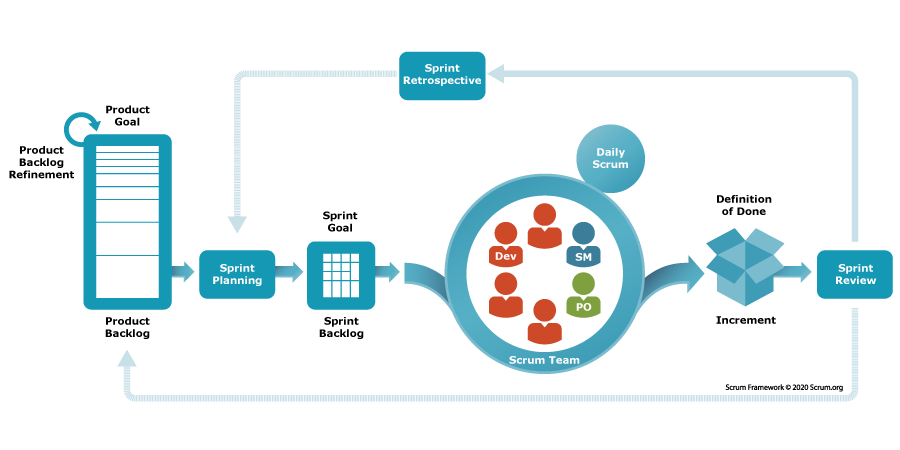
\includegraphics[width=0.8\linewidth]{BCS-Tessi/images/scrum_flow.png}
        \caption{Diagramma del flusso di lavoro del modello Scrum, basato sulla filosofia Agile}
        \label{fig:scrum_flow}
    \end{figure}
    
    \section{Organizzazione interna}
    SogeaSoft S.r.l. implementa i principi della norma \textbf{UNI EN ISO 9001:2015} per garantire un sistema di gestione della qualità dei prodotti efficace.
    
    \noindent Pur non essendo specificamente pensata per lo sviluppo \textit{software}, la norma trova applicazione nell’organizzazione grazie all’adozione di pratiche volte a standardizzare i processi e migliorare l’efficienza operativa. L'azienda basa la propria struttura sull'approccio per processi, suddividendo il lavoro in unità specializzate (come SAI, SAIPro e SAICon) e adottando metodologie \textit{Agile} per la pianificazione e gestione delle attività, ispirandosi allo standard ISO/IEC/IEEE 12207 (\textit{Systems and software engineering - Software life cycle processes}).

    \noindent Anche i principi dell’approccio per processi e del metodo Plan-Do-Check-Act (PDCA) sono applicati in tutte le fasi operative. Il PDCA si concretizza attraverso la pianificazione accurata delle attività (Plan), la loro esecuzione (Do), l’analisi dei risultati ottenuti (Check) e l’implementazione di eventuali azioni correttive o migliorative (Act).

    \noindent Un esempio evidente dell’applicazione del PDCA è riscontrabile nel modello di sviluppo Scrum, adottato da SogeaSoft S.r.l.per garantire iterazioni rapide e flessibili. Durante gli \textit{Sprint}, il \textit{backlog} viene pianificato e raffinato (\textit{Plan}), le attività vengono eseguite secondo le priorità stabilite (\textit{Do}), e i risultati sono presentati e analizzati attraverso la \textit{Sprint Review} e la \textit{Retrospective} (\textit{Check}). Eventuali miglioramenti vengono quindi incorporati negli \textit{Sprint} successivi (\textit{Act}).
    
    \noindent La Figura 1.3 mostra il certificato UNI EN ISO 9001:2015 ottenuto dall’azienda, che conferma l’impegno di SogeaSoft S.r.l. nel mantenere elevati standard di qualità nei propri processi.

    \begin{figure}[H]
        \centering
        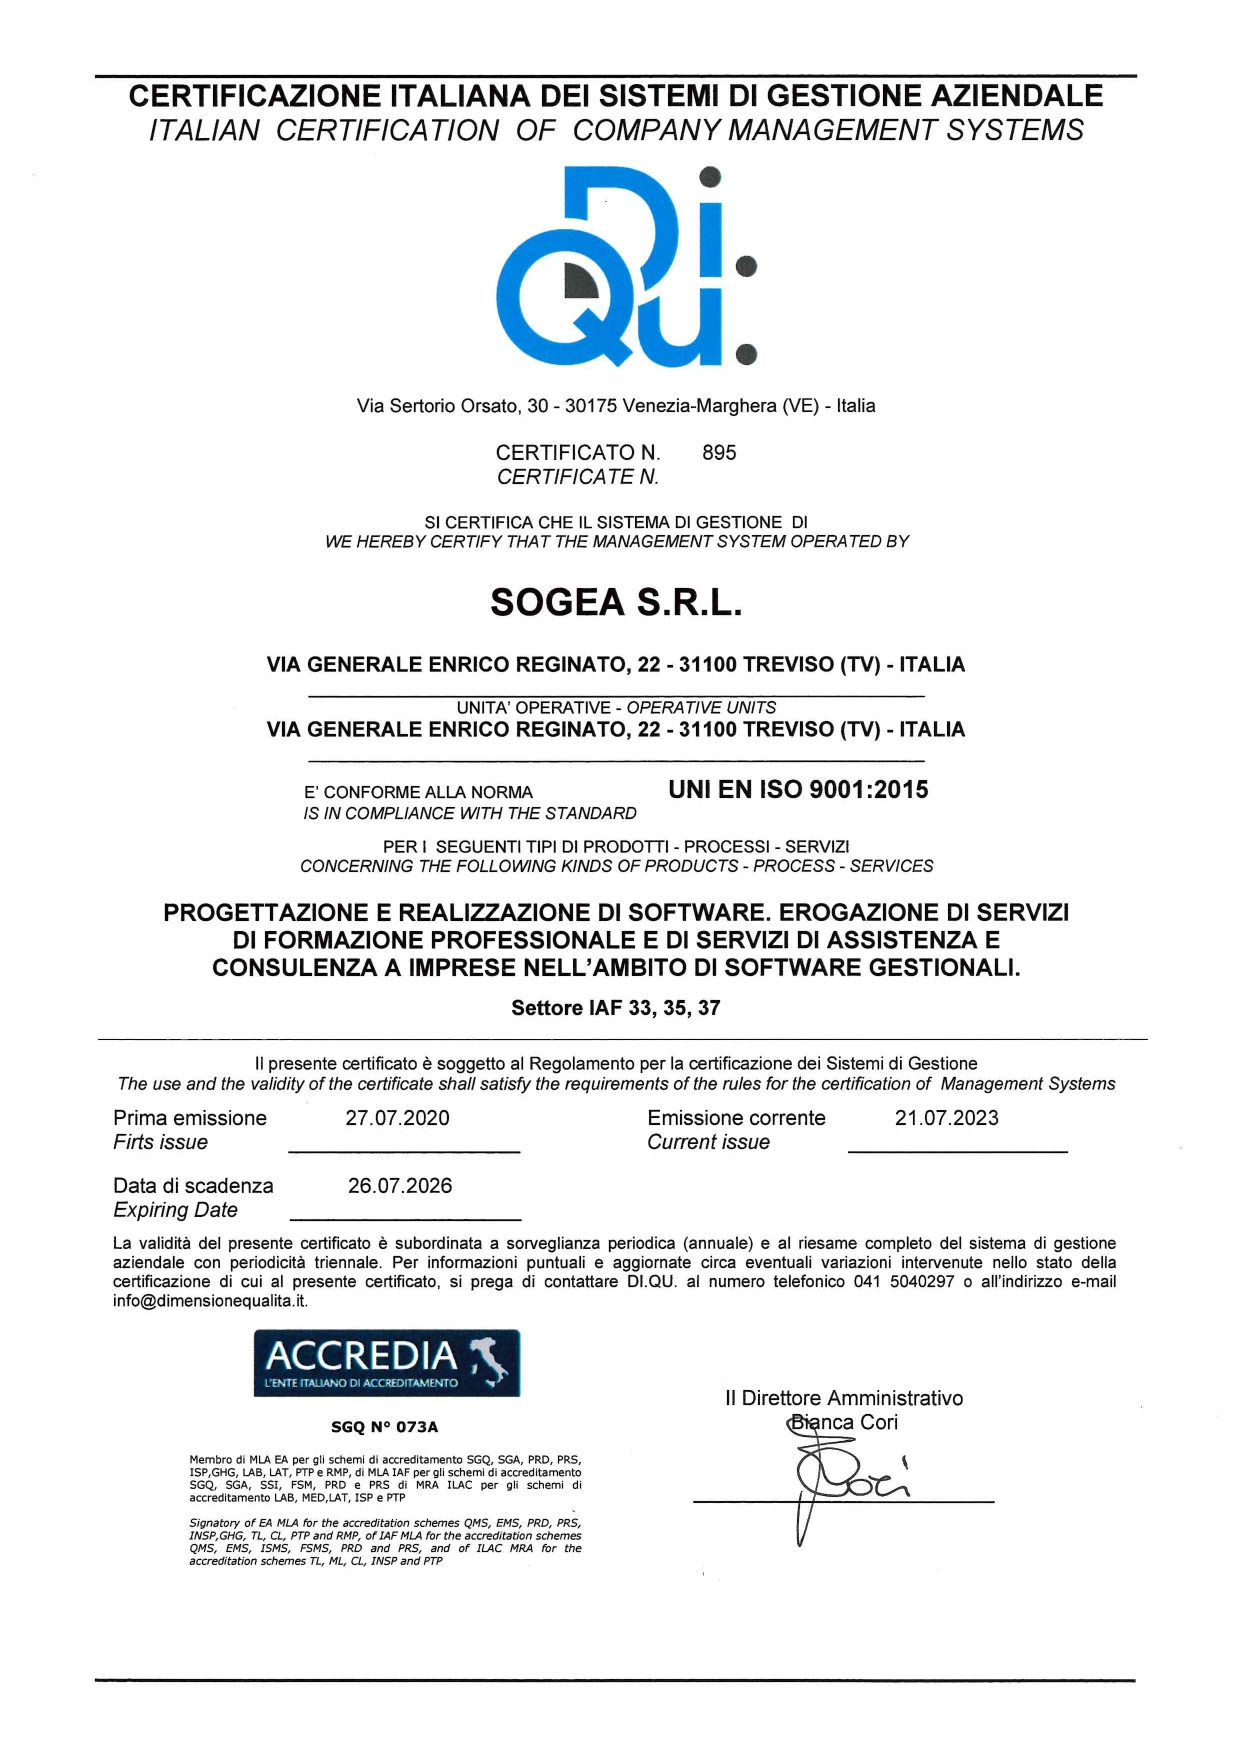
\includegraphics[width=0.5\linewidth]{BCS-Tessi/images/CertificatoSogea.jpg}
        \caption{Figura 1.3: Certificazione ISO ottenuta da SogeaSoft S.r.l.
        Fonte: https://sogeasoft.com/p/iso9001 \textit{(ultimo accesso 26/02/2025)}}
        \label{fig:certificazione-iso}
    \end{figure}

    \noindent Nelle successive sezioni approfondirò i processi di ciclo di vita del \textit{software} a cui ho avuto modo di partecipare durante il mio \textit{stage}. In particolare, riferendomi allo standard ISO/IEC/IEEE 12207:2017 tratterò i seguenti capitoli: Processi organizzativi e abilitanti e Processi di Gestione Tecnica.
    
    
        \subsection{Gestione della configurazione}
        Lo scopo del processo di Gestione della configurazione è stabilire e mantenere l'integrità di tutti gli \textit{output} identificati di un progetto o processo e renderli disponibili alle parti interessate. (ref: iso/iec)\\
        \noindent Nello specifico, un sistema di controllo è importante nell'evoluzione delle funzionalità del software, del codice e della documentazione associata perché essi costituiscono gli \textit{output} in questione. Ciò permette di mantenere traccia delle modifiche e garantire che ogni versione sia controllata, riproducibile e coerente con i requisiti stabiliti, facilitando così la gestione delle evoluzioni del \textit{software} e la collaborazione tra i membri del \textit{team}. 

        \noindent In SogeaSoft S.r.l. il controllo delle modifiche al codice avviene attraverso un \textit{Version Control System} (VCS), che traccia l’evoluzione del \textit{software} in modo strutturato. Le versioni del codice vengono archiviate all’interno di \textit{repository}, strutture dati appositamente organizzate per gestire i cambiamenti. 
        \noindent Queste \textit{repository} si basano su tre principali tipologie di \textit{branch}:  
        \begin{itemize}
            \item \textbf{master}: rappresenta la versione stabile destinata alla produzione, aggiornata manualmente in concomitanza con ogni rilascio ufficiale e avanzamento di versione; 
            \item \textbf{develop}: funge da \textit{branch} principale per lo sviluppo, raccogliendo le nuove funzionalità prima della loro distribuzione al Cliente; 
            \item \textbf{release}: include i \textit{branch} dedicati ai rilasci personalizzati, specifici per ogni cliente.  
        \end{itemize}

        \noindent La documentazione viene gestita all'interno di un'area dedicata dell'ambiente di sviluppo adottato (Sezione 1.5.2) da SogeaSoft S.r.l., denominata Wiki. Questo sistema organizza le informazioni in base ad argomenti, capitoli e finalità d'uso, garantendo una struttura relativamente chiara. Inoltre, ogni modifica è accompagnata da un \textit{timestamp} e dall'identificativo dell'autore, permettendo un tracciamento preciso delle revisioni. 
        
        \subsection{Gestione dell’informazione}

        Lo scopo del Processo di Gestione delle Informazioni è garantire alle parti designate l’accesso a informazioni pertinenti, tempestive, complete e valide durante e, ove opportuno, dopo il ciclo di vita del sistema (ref. ISO/IEC, par. 6.3.6).  

        \noindent Sogea S.r.l. impiega la piattaforma Microsoft Azure sia per la scrittura del codice sia per la gestione della documentazione aziendale. Questo strumento collaborativo facilita l'integrazione con diversi sistemi di supporto ai processi di Gestione della Configurazione, Progettazione, Implementazione e Manutenzione. In particolare, per la documentazione, SogeaSoft S.r.l. utilizza le Wiki, che consentono di organizzare e strutturare le informazioni in modo sistematico.  

        \begin{figure}[H]
            \centering
            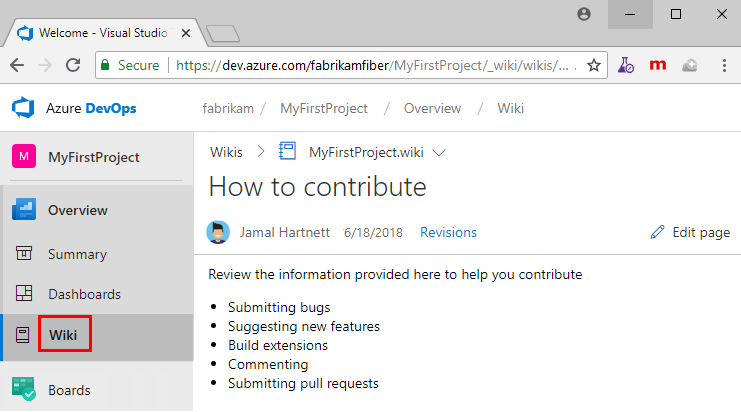
\includegraphics[width=0.5\linewidth]{BCS-Tessi/images/wiki_microsoft.png}
            \caption{Figura 1.4: Esempio di Wiki in Azure. Fonte: https://learn.microsoft.com/it-it/azure/devops/project/wiki/wiki-create-repo?view=azure-devopstabs=browser \textit{(ultimo accesso 1/03/2025)}}
            \label{fig:Wiki}
        \end{figure}

        \noindent Durante il mio \textit{stage}, ho osservato come, data l’interoperabilità del \textit{software} aziendale, risulti fondamentale che la documentazione associata sia formalmente strutturata in documenti accessibili a tutti i membri dei \textit{team}. Tale documentazione segue una gerarchia ben definita, comprendente la registrazione di incontri, requisiti, analisi e scelte progettuali, tutte adeguatamente descritte e motivate.  

        \noindent Tuttavia, questo approccio non è sempre stato adottato in maniera sistematica. Nelle versioni più datate del \textit{software}, la documentazione risultava spesso incompleta o assente, costringendo gli sviluppatori a ricorrere al \textit{reverse engineering} per comprendere il funzionamento del codice. Questa criticità ha generato una forte dipendenza dalle conoscenze dei singoli sviluppatori coinvolti nel processo iniziale, rendendo più complesso l’apporto di modifiche e aggiornamenti successivi.  

        \noindent Da qui deriva la necessità di SogeaSoft S.r.l. di abbandonare gradualmente il vecchio sistema in favore di un nuovo sistema più documentato, decentralizzato e flessibile. 
        
        \subsection{Processi di formazione}

        Durante il mio stage ho avuto modo di analizzare le modalità adottate da SogeaSoft S.r.l. per la formazione dei propri dipendenti. L'azienda implementa un approccio articolato, combinando diverse metodologie formative per garantire un apprendimento efficace e continuo. In particolare, le strategie impiegate comprendono:

        \begin{enumerate}
        \item \textbf{Lezioni in presenza}: nel caso in cui l’azienda intenda introdurre nuove tecnologie o apportare modifiche significative ai \textit{software} in uso, vengono organizzati corsi di formazione condotti da esperti del settore.

        \item \textbf{Autoapprendimento}: successivamente alle lezioni frontali, i dipendenti sono incoraggiati a integrare e approfondire autonomamente le conoscenze acquisite. Tale processo avviene attraverso la consultazione di libri tecnici, la visione di videolezioni su piattaforme online gratuite e l’analisi di progetti preesistenti affini.

        \item \textbf{Peer programming}: questa pratica collaborativa prevede il coinvolgimento di due o più programmatori nella scrittura del codice, promuovendo la condivisione di competenze e il miglioramento della qualità del \textit{software}. Solitamente, essa si concretizza nell’affiancamento di un programmatore esperto a uno meno esperto, con l’obiettivo di favorire un apprendimento diretto e pratico secondo il principio del \textit{learn by doing}.
        \end{enumerate}
        
        \noindent Nel corso del mio stage ho applicato prevalentemente le metodologie di \textbf{autoapprendimento} e \textit{\textbf{peer programming}}. Come si può osservare in Figura 1.5, nelle prime settimane la ricerca autonoma di informazioni e il confronto diretto con colleghi più esperti hanno occupato gran parte della mia giornata lavorativa. Tuttavia, con il progressivo consolidamento delle competenze acquisite, dopo circa dieci giorni lavorativi ho potuto ridurre significativamente il tempo dedicato allo studio individuale, limitando il ricorso al \textit{peer programming} ai soli casi in cui si presentassero difficoltà specifiche nello sviluppo del \textit{software}.

        \begin{figure} [H]
            \centering
            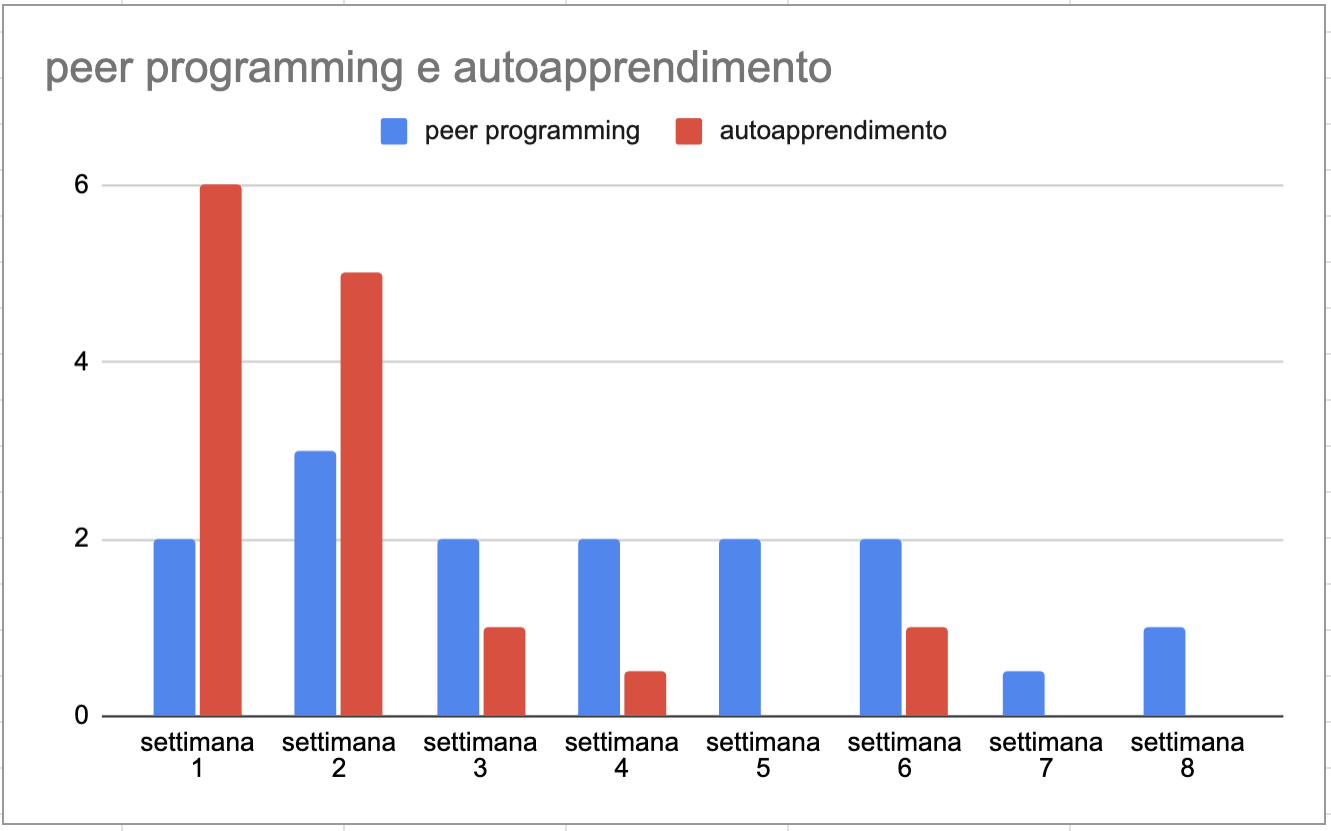
\includegraphics[width=0.8\linewidth]{BCS-Tessi/images/Ore_formazione.png}
            \caption{Rendicontazione ore (al giorno) dedicate ai processi di formazione durante il mio stage}
            \label{fig:Ore-formazione}
        \end{figure}
        

    \section{Ciclo di vita di un progetto software}
    Il ciclo di vita di un progetto \textit{software} rappresenta l’insieme delle fasi attraverso cui un sistema viene ideato, sviluppato, verificato e mantenuto nel tempo. Nell’ambito dello sviluppo \textit{Agile}, tale processo assume una natura iterativa e incrementale, consentendo una maggiore flessibilità nell’adattamento ai requisiti in evoluzione e nell’ottimizzazione continua del prodotto. Lo standard SO/IEC 12207 fornisce un quadro di riferimento formale per la gestione del ciclo di vita del \textit{software}, delineando attività strutturate per la pianificazione, lo sviluppo e la manutenzione. Le sezioni successive approfondiranno le principali fasi del ciclo di vita del software nel contesto aziendale di SogeaSoft S.r.l., con particolare riferimento all’esperienza maturata durante il mio \textit{stage}.
        \subsection{Analisi preliminare e raccolta dei requisiti}
        L’analisi dei bisogni degli \textit{stakeholder} e la raccolta dei requisiti rappresentano fasi fondamentali nel ciclo di vita di un progetto \textit{software}, poiché definiscono le basi su cui verrà sviluppato il sistema. Secondo lo standard ISO/IEC 12207, tali attività rientrano nel processo di gestione dei requisiti e hanno l’obiettivo di identificare, documentare e validare le esigenze delle parti interessate, garantendo che il \textit{software} finale sia allineato alle aspettative degli utenti. 

        \noindent Gli stakeholder di un progetto software possono includere clienti, utenti finali, team di sviluppo, responsabili di prodotto e altre figure coinvolte nel ciclo di vita del sistema. L’analisi dei bisogni si concentra sull’identificazione delle problematiche esistenti, sulle necessità operative e sugli obiettivi strategici che il software deve supportare. Tale attività si avvale di tecniche come interviste, workshop, focus group, questionari e l’osservazione diretta dei processi aziendali.

        Nel contesto dello sviluppo \textit{Agile}, questa fase è dinamica e continua: i bisogni vengono esplorati progressivamente, attraverso interazioni frequenti con gli \textit{stakeholder}. Per favorire la collaborazione costante con il \textit{Product Owner}, il quale agisce come intermediario tra il team di sviluppo e le parti interessate, assicurando che le priorità del prodotto riflettano i reali bisogni dell’azienda.

        Una volta analizzati i bisogni, si procede con la definizione e la formalizzazione dei requisiti, ovvero le specifiche funzionali e non funzionali che il software dovrà soddisfare. I requisiti funzionali descrivono le capacità e le operazioni del sistema, mentre quelli non funzionali riguardano aspetti come prestazioni, sicurezza, usabilità e scalabilità.

        Nello specifico SogeaSoft S.r.l. applica il concetto di Domain-Driven Design (DDD), un approccio che permea l’intero ciclo di vita dello sviluppo software, contribuendo a modellare il dominio in maniera coerente e a garantire che il sistema sviluppato risponda in modo preciso e scalabile alle esigenze precedentemente identificate.
        Nel contesto dell'analisi dei requisiti, l'introduzione di DDD comporta diversi passaggi chiave:

        \begin{itemize}
        \item Collaborazione con gli esperti del dominio (domain experts): L’elemento distintivo di DDD è il coinvolgimento continuo degli esperti del dominio, che sono coloro che possiedono una conoscenza approfondita del contesto in cui il sistema deve operare. Durante l'analisi dei requisiti, il team di sviluppo e gli esperti di dominio lavorano a stretto contatto per assicurarsi che i requisiti non siano solo funzionali, ma riflettano una comprensione profonda delle dinamiche del business.

        \item Creazione di un linguaggio comune (Ubiquitous Language): Uno degli aspetti centrali di DDD è l’adozione di un linguaggio comune, che consente a tutte le parti coinvolte nel progetto (sia tecniche che non tecniche) di discutere in modo chiaro e preciso i concetti chiave del dominio. Questo linguaggio deve essere utilizzato sin dalla fase di analisi dei requisiti per evitare ambiguità e garantire che tutti i requisiti siano ben definiti. Le User Stories possono essere redatte utilizzando il linguaggio condiviso, facilitando la comprensione tra gli stakeholder e il team di sviluppo.

        \item Definizione di Bounded Contexts: Un altro concetto fondamentale di DDD è la divisione del dominio in Bounded Contexts. Durante l'analisi dei requisiti, i team identificano e definiscono questi contesti limitati, ciascuno con il proprio modello di dominio, che può evolvere in modo indipendente dagli altri. Questo aiuta a evitare conflitti tra requisiti di diverse parti del sistema e facilita la gestione della complessità, permettendo di concentrarsi su una parte specifica del dominio alla volta.
        \end{itemize}

        In conclusione, l’integrazione del Domain-Driven Design nell’analisi dei requisiti consente di sviluppare un modello del dominio solido e coerente, facilitando la comunicazione tra gli stakeholder e il team di sviluppo. L’adozione di un linguaggio comune e la definizione di Bounded Contexts contribuiscono a ridurre le ambiguità e a migliorare l’allineamento tra le esigenze di business e le soluzioni software. Questo approccio favorisce non solo una progettazione più strutturata, ma anche una maggiore flessibilità nell’evoluzione del sistema, garantendo che il software possa adattarsi nel tempo alle mutevoli esigenze del dominio applicativo.
        \begin{figure} [H]
            \centering
            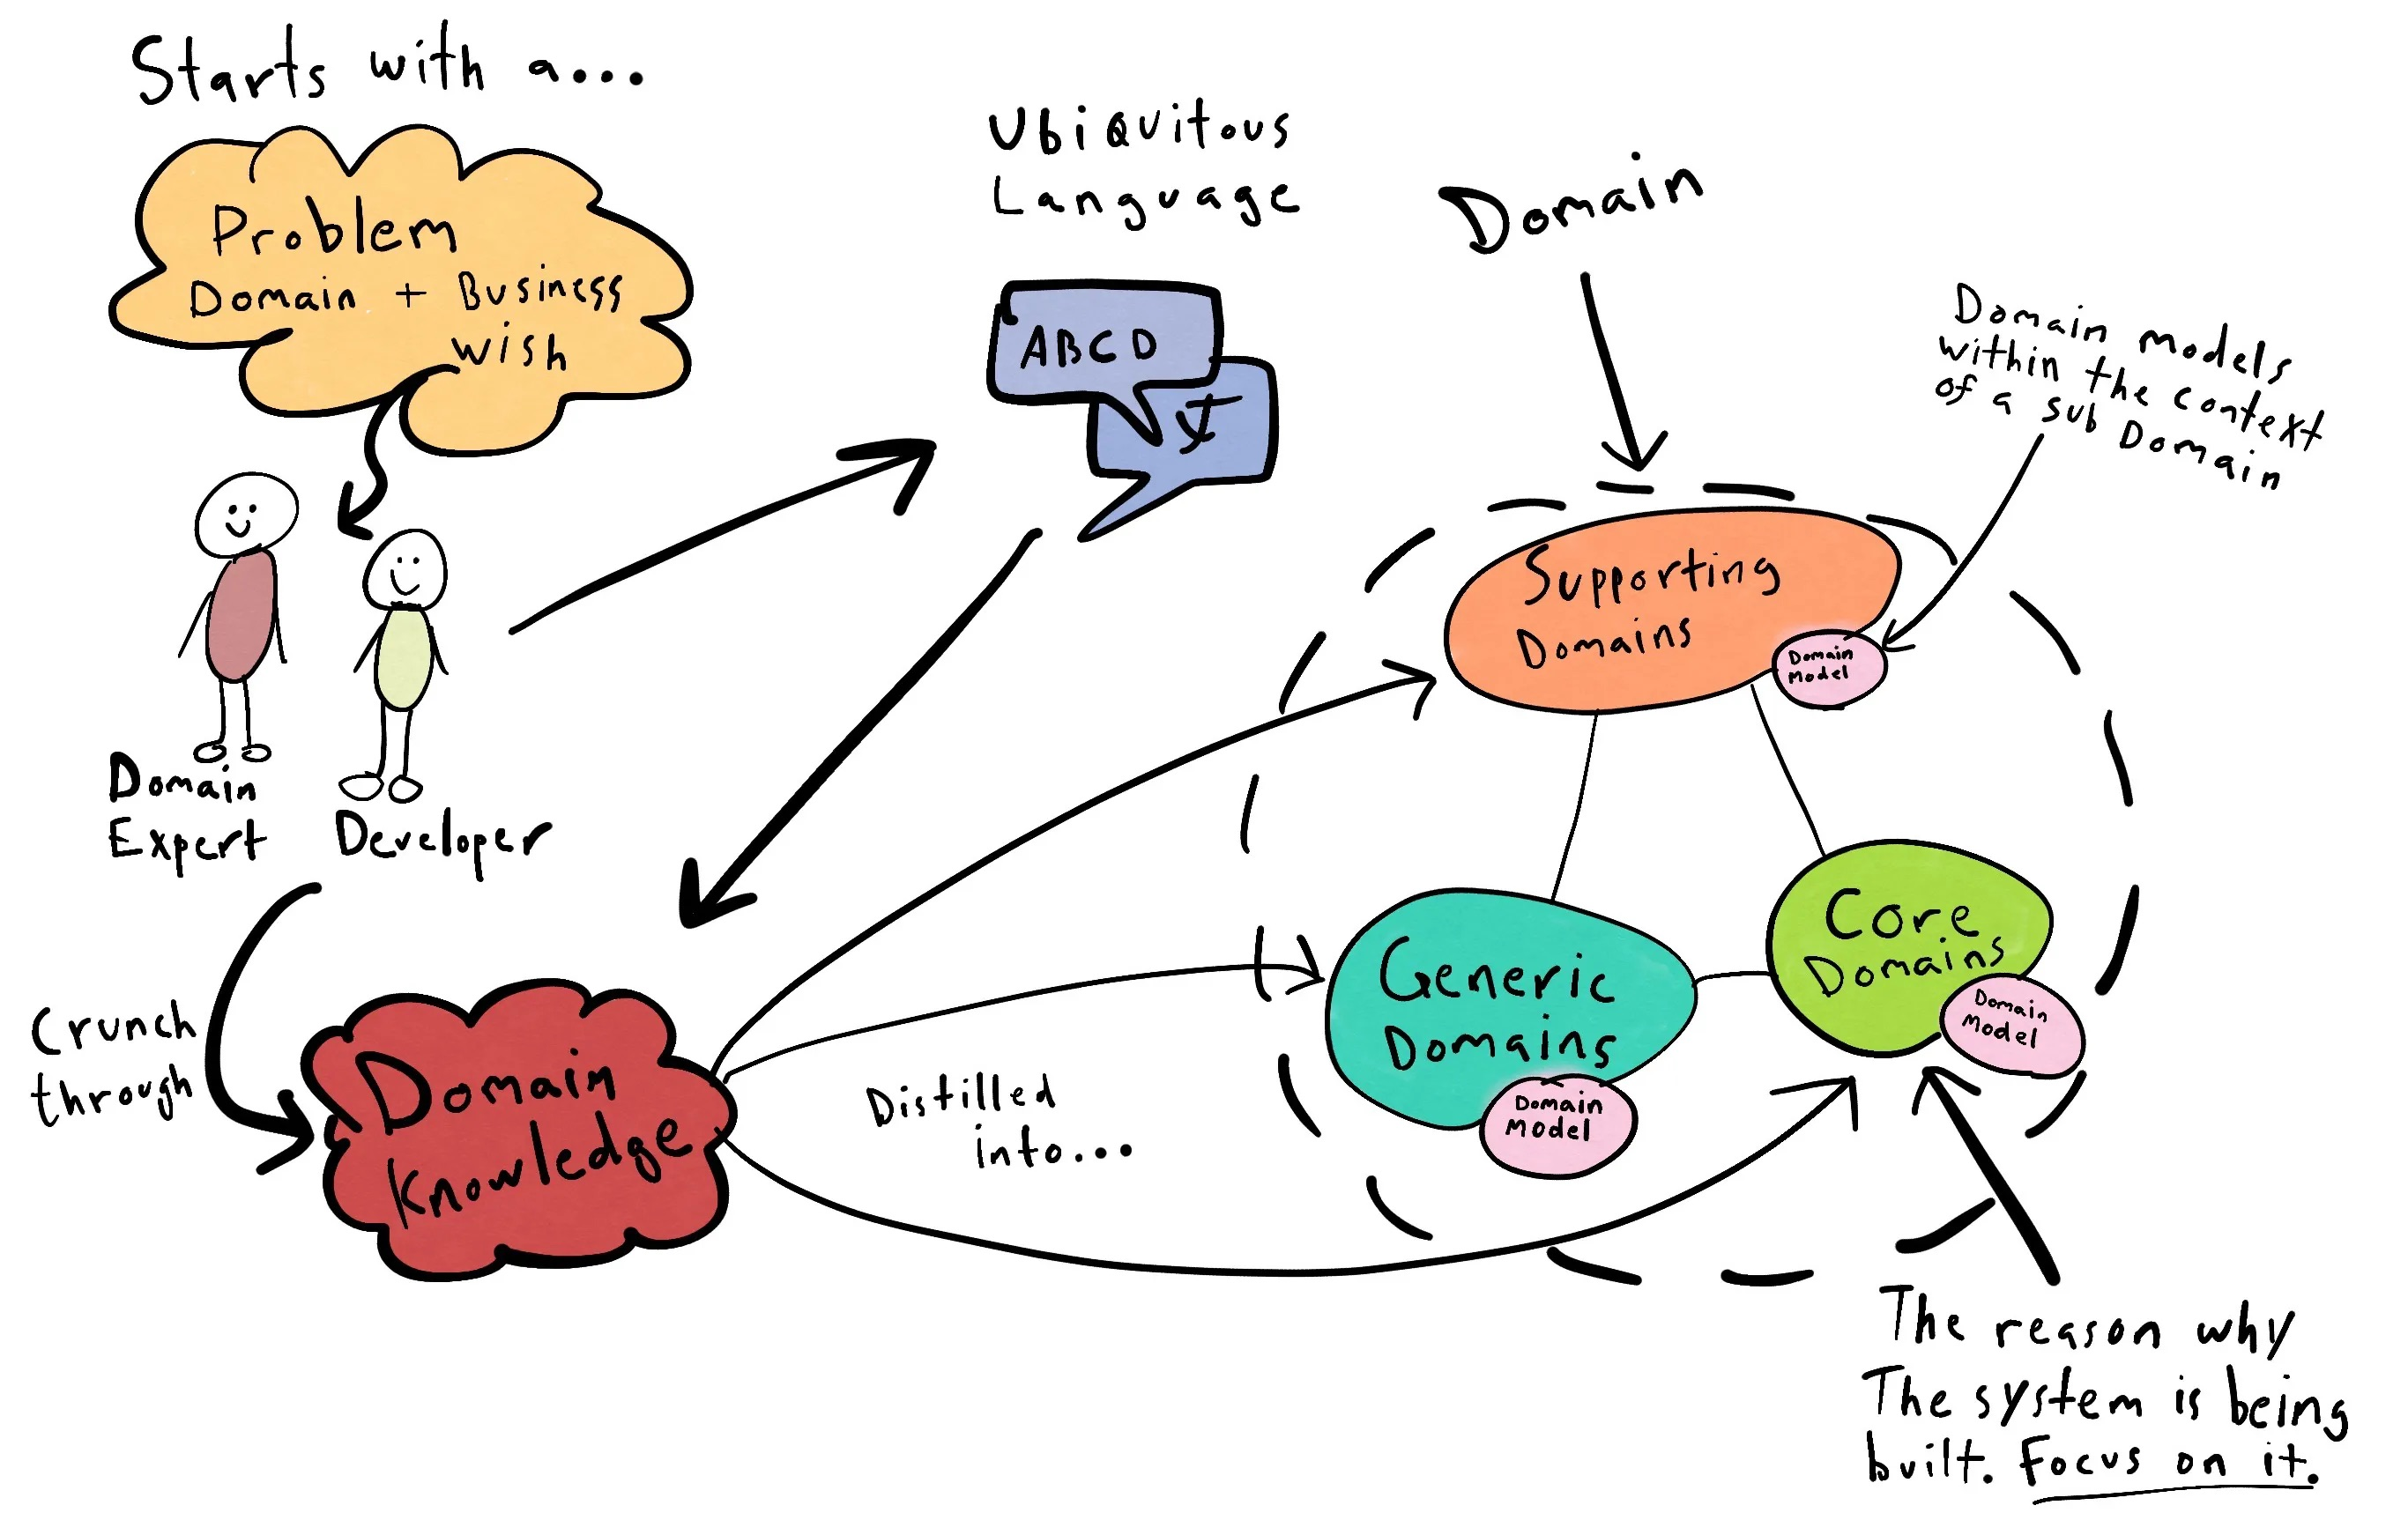
\includegraphics[width=0.7\linewidth]{BCS-Tessi/images/DDD_requisiti.jpeg}
            \caption{Figura 1.6: Visualizzazione del processo di analisi dei requisiti con DDD. Fonte :https://medium.com/raa-labs/part-1-domain-driven-design-like-a-pro-f9e78d081f10 (ultimo accesso 1/03/2025)}
            \label{fig:enter-label}
        \end{figure}
        
        \subsection{Progettazione}
        Il processo di progettazione software rappresenta una fase centrale del ciclo di vita dello sviluppo, in cui vengono definite l'architettura, i componenti e le interazioni del sistema al fine di garantire un’implementazione efficiente e conforme ai requisiti precedentemente raccolti. 
        Come previsto da Scrum (sezione 1.4), le attività di analisi e progettazione le abbiamo iterate, al fine di raggiungere soluzioni soddisfacenti. 
        In particolare, con l'approccio del Domain-Driven Design, introdotto nella sezione 1.6.1, abbiamo attuato le seguenti attività:
        Modellazione del dominio: Dopo aver raccolto i requisiti, la fase di progettazione è dove DDD inizia a entrare in gioco più attivamente. I team di sviluppo utilizzano il linguaggio comune e i concetti emersi durante l'analisi per costruire un modello di dominio dettagliato. In questa fase, vengono definiti gli aggregati, le entità, i valori e le funzioni di dominio. Gli aggregati rappresentano le entità principali del sistema che devono essere gestite come una singola unità per garantire la coerenza.
        Definizione degli eventuali microservizi: In un’architettura basata su microservizi, DDD aiuta a identificare e separare i Bounded Contexts in microservizi distinti, ciascuno con il proprio modello di dominio. Questo processo aiuta a mantenere una struttura chiara, riducendo la complessità e il rischio di conflitti tra le diverse parti del sistema.
        Pattern di progettazione: Nella progettazione, DDD sfrutta vari pattern architetturali e design patterns come il Repository Pattern, il Factory Pattern e il Specification Pattern, per creare un modello di dominio robusto, flessibile e facilmente estensibile.
        
        \subsection{Sviluppo}
        L'attività di implementazione costituisce una fase essenziale nel ciclo di vita del software, in cui la soluzione progettata viene tradotta in codice eseguibile, rendendola concretamente fruibile dagli utenti finali. Secondo lo standard ISO/IEC 12207, l'implementazione rientra nei processi primari di sviluppo e comprende la scrittura, la verifica e l'integrazione del codice, garantendo che il prodotto software soddisfi i requisiti definiti nelle fasi precedenti.

        Per la gestione e il monitoraggio delle attività di codifica, l'azienda SogeaSoft S.r.l. utilizza Microsoft Azure, una piattaforma che integra un Issue Tracking System (ITS). Questo strumento consente di gestire e tracciare le attività di sviluppo, offrendo una visione olistica del progetto sia dal punto di vista gestionale che implementativo. L'impiego di un ITS favorisce l'organizzazione del lavoro, prevenendo inefficienze e sovrapposizioni tra gli sviluppatori.

        Nel contesto del Domain-Driven Design (DDD), l’implementazione segue principi mirati a garantire la coerenza tra il modello concettuale del dominio e la struttura del codice. In particolare, la fase di sviluppo prevede la codifica del modello di dominio.
        Quest'ultimo, elaborato durante la fase di progettazione, viene tradotto in codice attraverso l'implementazione delle componenti individuate nella fase precedente. Tali componenti vengono strutturate in modo da rispettare le regole di business definite in precedenza, utilizzando il linguaggio comune (Ubiquitous Language) condiviso tra gli stakeholder per assicurare consistenza semantica.
        
        All'interno di SogeaSoft S.r.l., l'attività di sviluppo è organizzata mediante un sistema di task assignment, in cui ogni attività (detta anche Issue) viene assegnata a uno sviluppatore specifico. Questo approccio favorisce un’elevata ownership del lavoro, responsabilizzando il singolo sviluppatore e ottimizzando la gestione delle risorse.

        A seconda del livello di urgenza e priorità, il Team Leader può collocare l’attività di implementazione all’interno dello Sprint Backlog, qualora si tratti di una lavorazione prioritaria, oppure nel Product Backlog, in attesa di essere raffinata e pianificata nei successivi incontri di Raffinamento del backlog.

        Lo sviluppo del codice avviene secondo una strategia di version control strutturata: per ogni attività assegnata, viene creato un branch dedicato a partire dal ramo di sviluppo principale (develop). Tale branch viene nominato seguendo una convenzione specifica, includendo parole chiave come "feature" (nuova funzionalità) o "bug-fix" (correzione di errori), seguite da una breve descrizione dell’attività, al fine di garantire una chiara identificazione e tracciabilità delle modifiche.


        Una volta completata la fase di codifica, il codice prodotto è sottoposto a un processo di verifica e validazione (Sezione 1.6.4), il quale si concretizza nell'apertura di una Pull Request (PR). Tramite la PR, lo sviluppatore richiede una revisione formale delle modifiche da parte del Team Leader o di un altro membro del team con pari competenze. Solo a seguito della validazione, il codice viene integrato nella codebase principale attraverso un'operazione di merge nel repository del progetto, garantendo così il mantenimento della qualità del software e la coerenza dell’intero sistema.

        
        \subsection{Verifica e Validazione}
        Il processo di verifica ha l’obiettivo di fornire evidenza oggettiva della capacità del software di soddisfare i requisiti e le caratteristiche definite. Durante il mio periodo di osservazione, ho avuto l'opportunità di assistere da vicino all'esecuzione delle attività legate a questo processo.

La **verifica del software** si svolge in più fasi, partendo dalle singole unità di codice fino ad estendersi al sistema nel suo complesso. Le principali tipologie di test utilizzate sono le seguenti:

- **Test di unità**: questi test verificano le singole unità di codice, ovvero porzioni atomiche e eseguibili che espongono un comportamento specifico. Il framework **Synergy** prevede la generazione automatica di alcuni test unitari, sebbene si tratti principalmente di test di tipo triviale, che si limitano a controllare la gestione dei tipi di dati e delle eccezioni. La maggior parte dei test unitari che ho sviluppato ha riguardato invece i comportamenti definiti dai requisiti individuati durante la fase di progettazione.

- **Test di integrazione**: questi test verificano il comportamento e l'interazione tra le diverse parti del sistema, assicurandosi che il software rispetti i requisiti funzionali previsti.

- **Test di sistema**: questi test mirano a verificare la conformità del software nel suo insieme, considerando le dipendenze tra le varie componenti. In questo caso, la gestione delle dipendenze è affidata allo strumento **Gradle**, che facilita l’integrazione e l’esecuzione dei test a livello di sistema.

Il processo di Validazione14 fornisce evidenza oggettiva sulla capacità del software di soddisfare le aspettative e i bisogni del committente, sia esso esterno (ovvero un’azienda cliente) o interno (ovvero una BU di Sanmarco Informatica S.p.A.).
Durante le prime settimane di stage, la validazione dei risultati delle mie attività (modesti per impatto) spettava ad un Solution Developer.
 Tuttavia, la validazione delle funzionalità avviene solitamente da parte del Product Owner, durante gli Sprint Grooming o le Sprint Review. In questo modo, si può concentrare in un’unico incontro la maggior parte delle attività di validazione e, in caso di incongruenze, allineare tutto il team ai requisiti.
In taluni casi, ho avuto la possibilità di partecipare ai meeting di validazione con i rappresentanti delle aziende clienti.
La validazione, positiva o negativa, è sempre registrata nei relativi documenti di tracciamento, assieme al feedback ottenuto.

SogeaSoft S.r.l. adotta un processo di verifica e validazione strutturato, seppur con una metodologia flessibile. La scrittura di test non è obbligatoria per la presentazione e la validazione del software. Tuttavia, quando presenti, i test vengono sviluppati direttamente all’interno dell'ambiente DevOps, sfruttando le sue pipeline. In questo ambiente, il codice viene compilato e i test vengono eseguiti automaticamente.

Questi test vengono eseguiti sulle Pull Requests (PR) nei branch designati, garantendo che le modifiche apportate non introducano errori nel sistema. La validazione delle PR è un processo collaborativo che coinvolge più sviluppatori: i colleghi svolgono una revisione del codice e, salvo casi particolari, la validazione richiede l’approvazione di due revisori che non siano gli sviluppatori stessi delle modifiche. Questo processo assicura una maggiore qualità del codice e riduce i rischi di errori, mantenendo alta la coerenza del prodotto software.
        
        \subsection{Manutenzione}
Il processo di Manutenzione15 ha lo scopo di sostenere la capacità del software di essere usabile, e cioè di soddisfare bisogni e requisiti, anche postumi, dal momento della distribuzione fino al suo ritiro.
Ciò avviene mediante azioni correttive o migliorative, attuate in modo adattivo (ad esempio, dopo una segnalazione di malfunzionamento) o preventivo (ad esempio, dopo aver individuato internamente ambiti di miglioramento). Lo sviluppo del software, infatti, non termina con la sua pubblicazione, ma prosegue per tutta la sua vita utile. Molti dei software venduti da Sanmarco Informatica S.p.A. sono in uso da decenni e vengono tuttora aggiornati regolarmente: ciò non sarebbe possibile con una cattiva gestione del debito tecnico.
I software di Factory sono largamente utilizzati in moltissime nicchie dei settori manifatturiero e logistico e, pertanto, sono soggetti a frequenti richieste di cambiamento. La fonte di tali richieste può essere:
• esterna, ovvero proveniente da un Cliente: in questo caso, può trattarsi di una richiesta di
manutenzione correttiva (ad esempio per la rimozione di un bug ), oppure di aggiunta di nuove
funzionalità o ancora di evoluzione delle funzionalità già presenti;
• interna, ovvero proveniente da una BU: la richiesta pervenuta può mirare:
– al miglioramento della sicurezza o delle prestazioni del software;
– all’aggiornamento delle tecnologie abilitanti su cui si basa Synergy;
– all’introduzione di nuove funzionalità, individuate tramite ricerche interne, atte ad aumentare
la competitività dei prodotti.
È importante ricordare che la manutenzione è un costo. Pertanto, è cruciale garantire la manutenibilità del software prodotto, sia tramite l’adozione di buone pratiche di codifica (Sezione 1.5.3.3), che tramite la produzione di documentazione precisa, aggiornata e attendibile (Sezione 1.5.2.2).

        Evoluzione del modello: Il DDD non è un approccio che si ferma alla fase di progettazione e implementazione. Dopo la messa in produzione del software, il modello di dominio potrebbe evolversi man mano che emergono nuove esigenze o nuove informazioni. Poiché DDD enfatizza un approccio iterativo e incrementale, è possibile aggiornare e migliorare il modello di dominio attraverso il feedback degli utenti o la scoperta di nuove parti del dominio.
Adattamento ai cambiamenti del dominio: Nel corso del tempo, possono verificarsi cambiamenti nelle esigenze aziendali. DDD facilita l'adattamento del sistema a tali cambiamenti, mantenendo un forte allineamento con il business. Durante la manutenzione, è possibile rivedere i Bounded Contexts e le interfacce tra i vari modelli di dominio, migliorando la separazione delle preoccupazioni.
    \section{Tecnologie utilizzate}
    Per la realizzazione dei suoi prodotti, la BU Factory di Sanmarco Informatica S.p.A. impiega un insieme di tecnologie predefinito e comune a tutti i software sviluppati. Riporto esclusivamente ciò di cui ho avuto esperienza diretta durante il periodo di stage: si tratta di una selezione di tecnologie, strumenti e servizi con licenze d’uso diverse, che assieme costituiscono lo stack tecnologico del framework Synergy.
I linguaggi di programmazione utilizzati sono:


    Scriverò una descrizione dettagliata di tutte le tecnologie utilizzate dall’azienda specificamente nello
    sviluppo software. Ai fini di questa trattazione descriverò anche le tecnologie obsolete che non sono
    più utilizzate dai dipendenti ma che sono ancora in uso nei meandri del prodotto principale
    dell’azienda SogeaSoft S.r.l.
    Nello specifico descriverò: linguaggi di programmazione, tecnologie alla base dei prodotti
    d   ell’azienda, l’ambiente di sviluppo, gli editor utilizzati, e       strumenti per i processi di verifica.
    \section{L’innovazione in Sogea}

    SogeaSoft S.r.l. ha dimostrato una propensione all'innovazione che, pur non essendo caratterizzata da un approccio radicale, si è sviluppata in maniera progressiva e riflessiva. Inizialmente, l'azienda ha adottato un modello di evoluzione del prodotto che seguiva un processo iterativo, dove le modifiche e le migliorie venivano introdotte step-by-step. Questo approccio, pur offrendo una certa stabilità, rifletteva una cautela nell'adozione di nuove tecnologie, in parte dovuta a preoccupazioni relative ai rischi associati a cambiamenti rapidi e non completamente testati.

Nonostante tale prudenza iniziale, SogeaSoft ha saputo sviluppare nel tempo un framework solido e aggiornato, soprattutto per quanto riguarda la gestione dei progetti, che si è adattato alle esigenze emergenti nel settore. In particolare, la parte relativa al sistema ERP (Enterprise Resource Planning) ha subito una lenta ma continua evoluzione, con l'obiettivo di rispondere alle nuove necessità aziendali senza compromettere la stabilità operativa. La transizione verso l'aggiornamento di tale componente è stata attentamente ponderata, con un'analisi costante delle potenzialità offerte da tecnologie emergenti e delle risorse necessarie per implementarle in modo efficace.

Sebbene l'azienda non abbia intrapreso l'adozione di innovazioni radicali, la sua capacità di evolversi in modo costante e sostenibile ha permesso a SogeaSoft di mantenere una posizione competitiva nel mercato. L'approccio adottato, che prevede l'allocazione di risorse umane e finanziarie in base alla necessità percepita, ha favorito l'implementazione di miglioramenti incrementali, garantendo una continua crescita della capacità produttiva e un aggiornamento costante della tecnologia utilizzata. 

Tuttavia, è evidente che la sua strategia innovativa, seppur efficace, si è sempre mantenuta prudente rispetto a quelle di aziende che sono nate più recentemente, spesso con una mentalità più orientata all'adozione rapida di nuove tecnologie. Queste ultime, infatti, pur disponendo di un prodotto giovane, hanno avuto la possibilità di svilupparsi con tecnologie moderne sin dall'inizio, facendo leva su un approccio innovativo più audace. La differenza fondamentale risiede nella volontà di SogeaSoft di integrare l'innovazione in modo graduale, prendendo in considerazione non solo le opportunità tecnologiche ma anche i rischi operativi e finanziari.
    Scriverò una descrizione accurata della propensione all’innovazione di Sogea, spiegando le concrete
    misure che l’azienda sta adottando a tal proposito. Includerò come Bluenext abbia contribuito in ciò.

    Questo è un esempio di citazione\footnote{\small Nome dell'autore, \emph{Titolo del libro}, Anno di pubblicazione, Editore.}.
